% Graphic for TeX using PGF
% Title: C:\Users\User\Google Drive\DEVS EX Machina\benchmarks\cores_class_diagram.dia
% Creator: Dia v0.97.2
% CreationDate: Wed Dec 09 16:57:11 2015
% For: User
% \usepackage{tikz}
% The following commands are not supported in PSTricks at present
% We define them conditionally, so when they are implemented,
% this pgf file will use them.
\ifx\du\undefined
  \newlength{\du}
\fi
\setlength{\du}{15\unitlength}
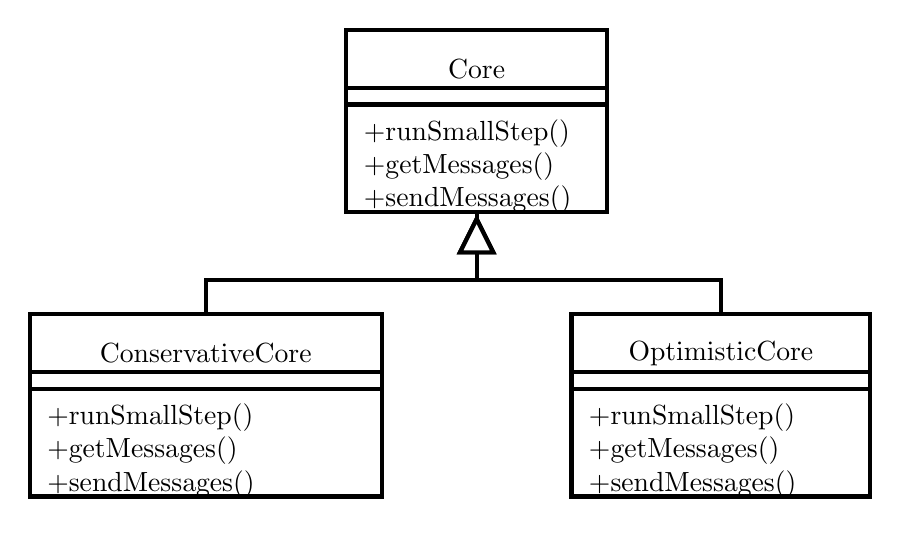
\begin{tikzpicture}
\pgftransformxscale{1.000000}
\pgftransformyscale{-1.000000}
\definecolor{dialinecolor}{rgb}{0.000000, 0.000000, 0.000000}
\pgfsetstrokecolor{dialinecolor}
\definecolor{dialinecolor}{rgb}{1.000000, 1.000000, 1.000000}
\pgfsetfillcolor{dialinecolor}
\pgfsetlinewidth{0.100000\du}
\pgfsetdash{}{0pt}
\definecolor{dialinecolor}{rgb}{1.000000, 1.000000, 1.000000}
\pgfsetfillcolor{dialinecolor}
\fill (22.402500\du,8.450000\du)--(22.402500\du,9.850000\du)--(28.677500\du,9.850000\du)--(28.677500\du,8.450000\du)--cycle;
\definecolor{dialinecolor}{rgb}{0.000000, 0.000000, 0.000000}
\pgfsetstrokecolor{dialinecolor}
\draw (22.402500\du,8.450000\du)--(22.402500\du,9.850000\du)--(28.677500\du,9.850000\du)--(28.677500\du,8.450000\du)--cycle;
% setfont left to latex
\definecolor{dialinecolor}{rgb}{0.000000, 0.000000, 0.000000}
\pgfsetstrokecolor{dialinecolor}
\node at (25.540000\du,9.400000\du){Core};
\definecolor{dialinecolor}{rgb}{1.000000, 1.000000, 1.000000}
\pgfsetfillcolor{dialinecolor}
\fill (22.402500\du,9.850000\du)--(22.402500\du,10.250000\du)--(28.677500\du,10.250000\du)--(28.677500\du,9.850000\du)--cycle;
\definecolor{dialinecolor}{rgb}{0.000000, 0.000000, 0.000000}
\pgfsetstrokecolor{dialinecolor}
\draw (22.402500\du,9.850000\du)--(22.402500\du,10.250000\du)--(28.677500\du,10.250000\du)--(28.677500\du,9.850000\du)--cycle;
\definecolor{dialinecolor}{rgb}{1.000000, 1.000000, 1.000000}
\pgfsetfillcolor{dialinecolor}
\fill (22.402500\du,10.250000\du)--(22.402500\du,12.850000\du)--(28.677500\du,12.850000\du)--(28.677500\du,10.250000\du)--cycle;
\definecolor{dialinecolor}{rgb}{0.000000, 0.000000, 0.000000}
\pgfsetstrokecolor{dialinecolor}
\draw (22.402500\du,10.250000\du)--(22.402500\du,12.850000\du)--(28.677500\du,12.850000\du)--(28.677500\du,10.250000\du)--cycle;
% setfont left to latex
\definecolor{dialinecolor}{rgb}{0.000000, 0.000000, 0.000000}
\pgfsetstrokecolor{dialinecolor}
\node[anchor=west] at (22.552500\du,10.950000\du){+runSmallStep()};
% setfont left to latex
\definecolor{dialinecolor}{rgb}{0.000000, 0.000000, 0.000000}
\pgfsetstrokecolor{dialinecolor}
\node[anchor=west] at (22.552500\du,11.750000\du){+getMessages()};
% setfont left to latex
\definecolor{dialinecolor}{rgb}{0.000000, 0.000000, 0.000000}
\pgfsetstrokecolor{dialinecolor}
\node[anchor=west] at (22.552500\du,12.550000\du){+sendMessages()};
\pgfsetlinewidth{0.100000\du}
\pgfsetdash{}{0pt}
\pgfsetmiterjoin
\pgfsetbuttcap
{
\definecolor{dialinecolor}{rgb}{0.000000, 0.000000, 0.000000}
\pgfsetfillcolor{dialinecolor}
% was here!!!
\definecolor{dialinecolor}{rgb}{0.000000, 0.000000, 0.000000}
\pgfsetstrokecolor{dialinecolor}
\draw (25.540000\du,12.900275\du)--(25.540000\du,14.472500\du)--(19.015000\du,14.472500\du)--(19.015000\du,15.244725\du);
}
\definecolor{dialinecolor}{rgb}{0.000000, 0.000000, 0.000000}
\pgfsetstrokecolor{dialinecolor}
\draw (25.540000\du,13.812078\du)--(25.540000\du,14.472500\du)--(19.015000\du,14.472500\du)--(19.015000\du,15.244725\du);
\pgfsetmiterjoin
\definecolor{dialinecolor}{rgb}{1.000000, 1.000000, 1.000000}
\pgfsetfillcolor{dialinecolor}
\fill (25.940000\du,13.812078\du)--(25.540000\du,13.012078\du)--(25.140000\du,13.812078\du)--cycle;
\pgfsetlinewidth{0.100000\du}
\pgfsetdash{}{0pt}
\pgfsetmiterjoin
\definecolor{dialinecolor}{rgb}{0.000000, 0.000000, 0.000000}
\pgfsetstrokecolor{dialinecolor}
\draw (25.940000\du,13.812078\du)--(25.540000\du,13.012078\du)--(25.140000\du,13.812078\du)--cycle;
% setfont left to latex
\pgfsetlinewidth{0.100000\du}
\pgfsetdash{}{0pt}
\pgfsetmiterjoin
\pgfsetbuttcap
{
\definecolor{dialinecolor}{rgb}{0.000000, 0.000000, 0.000000}
\pgfsetfillcolor{dialinecolor}
% was here!!!
\definecolor{dialinecolor}{rgb}{0.000000, 0.000000, 0.000000}
\pgfsetstrokecolor{dialinecolor}
\draw (25.540000\du,12.900275\du)--(25.540000\du,14.472500\du)--(31.425000\du,14.472500\du)--(31.425000\du,15.244725\du);
}
\definecolor{dialinecolor}{rgb}{0.000000, 0.000000, 0.000000}
\pgfsetstrokecolor{dialinecolor}
\draw (25.540000\du,13.812078\du)--(25.540000\du,14.472500\du)--(31.425000\du,14.472500\du)--(31.425000\du,15.244725\du);
\pgfsetmiterjoin
\definecolor{dialinecolor}{rgb}{1.000000, 1.000000, 1.000000}
\pgfsetfillcolor{dialinecolor}
\fill (25.940000\du,13.812078\du)--(25.540000\du,13.012078\du)--(25.140000\du,13.812078\du)--cycle;
\pgfsetlinewidth{0.100000\du}
\pgfsetdash{}{0pt}
\pgfsetmiterjoin
\definecolor{dialinecolor}{rgb}{0.000000, 0.000000, 0.000000}
\pgfsetstrokecolor{dialinecolor}
\draw (25.940000\du,13.812078\du)--(25.540000\du,13.012078\du)--(25.140000\du,13.812078\du)--cycle;
% setfont left to latex
\pgfsetlinewidth{0.100000\du}
\pgfsetdash{}{0pt}
\definecolor{dialinecolor}{rgb}{1.000000, 1.000000, 1.000000}
\pgfsetfillcolor{dialinecolor}
\fill (14.775000\du,15.295000\du)--(14.775000\du,16.695000\du)--(23.255000\du,16.695000\du)--(23.255000\du,15.295000\du)--cycle;
\definecolor{dialinecolor}{rgb}{0.000000, 0.000000, 0.000000}
\pgfsetstrokecolor{dialinecolor}
\draw (14.775000\du,15.295000\du)--(14.775000\du,16.695000\du)--(23.255000\du,16.695000\du)--(23.255000\du,15.295000\du)--cycle;
% setfont left to latex
\definecolor{dialinecolor}{rgb}{0.000000, 0.000000, 0.000000}
\pgfsetstrokecolor{dialinecolor}
\node at (19.015000\du,16.245000\du){ConservativeCore};
\definecolor{dialinecolor}{rgb}{1.000000, 1.000000, 1.000000}
\pgfsetfillcolor{dialinecolor}
\fill (14.775000\du,16.695000\du)--(14.775000\du,17.095000\du)--(23.255000\du,17.095000\du)--(23.255000\du,16.695000\du)--cycle;
\definecolor{dialinecolor}{rgb}{0.000000, 0.000000, 0.000000}
\pgfsetstrokecolor{dialinecolor}
\draw (14.775000\du,16.695000\du)--(14.775000\du,17.095000\du)--(23.255000\du,17.095000\du)--(23.255000\du,16.695000\du)--cycle;
\definecolor{dialinecolor}{rgb}{1.000000, 1.000000, 1.000000}
\pgfsetfillcolor{dialinecolor}
\fill (14.775000\du,17.095000\du)--(14.775000\du,19.695000\du)--(23.255000\du,19.695000\du)--(23.255000\du,17.095000\du)--cycle;
\definecolor{dialinecolor}{rgb}{0.000000, 0.000000, 0.000000}
\pgfsetstrokecolor{dialinecolor}
\draw (14.775000\du,17.095000\du)--(14.775000\du,19.695000\du)--(23.255000\du,19.695000\du)--(23.255000\du,17.095000\du)--cycle;
% setfont left to latex
\definecolor{dialinecolor}{rgb}{0.000000, 0.000000, 0.000000}
\pgfsetstrokecolor{dialinecolor}
\node[anchor=west] at (14.925000\du,17.795000\du){+runSmallStep()};
% setfont left to latex
\definecolor{dialinecolor}{rgb}{0.000000, 0.000000, 0.000000}
\pgfsetstrokecolor{dialinecolor}
\node[anchor=west] at (14.925000\du,18.595000\du){+getMessages()};
% setfont left to latex
\definecolor{dialinecolor}{rgb}{0.000000, 0.000000, 0.000000}
\pgfsetstrokecolor{dialinecolor}
\node[anchor=west] at (14.925000\du,19.395000\du){+sendMessages()};
\pgfsetlinewidth{0.100000\du}
\pgfsetdash{}{0pt}
\definecolor{dialinecolor}{rgb}{1.000000, 1.000000, 1.000000}
\pgfsetfillcolor{dialinecolor}
\fill (27.825000\du,15.295000\du)--(27.825000\du,16.695000\du)--(35.025000\du,16.695000\du)--(35.025000\du,15.295000\du)--cycle;
\definecolor{dialinecolor}{rgb}{0.000000, 0.000000, 0.000000}
\pgfsetstrokecolor{dialinecolor}
\draw (27.825000\du,15.295000\du)--(27.825000\du,16.695000\du)--(35.025000\du,16.695000\du)--(35.025000\du,15.295000\du)--cycle;
% setfont left to latex
\definecolor{dialinecolor}{rgb}{0.000000, 0.000000, 0.000000}
\pgfsetstrokecolor{dialinecolor}
\node at (31.425000\du,16.245000\du){OptimisticCore};
\definecolor{dialinecolor}{rgb}{1.000000, 1.000000, 1.000000}
\pgfsetfillcolor{dialinecolor}
\fill (27.825000\du,16.695000\du)--(27.825000\du,17.095000\du)--(35.025000\du,17.095000\du)--(35.025000\du,16.695000\du)--cycle;
\definecolor{dialinecolor}{rgb}{0.000000, 0.000000, 0.000000}
\pgfsetstrokecolor{dialinecolor}
\draw (27.825000\du,16.695000\du)--(27.825000\du,17.095000\du)--(35.025000\du,17.095000\du)--(35.025000\du,16.695000\du)--cycle;
\definecolor{dialinecolor}{rgb}{1.000000, 1.000000, 1.000000}
\pgfsetfillcolor{dialinecolor}
\fill (27.825000\du,17.095000\du)--(27.825000\du,19.695000\du)--(35.025000\du,19.695000\du)--(35.025000\du,17.095000\du)--cycle;
\definecolor{dialinecolor}{rgb}{0.000000, 0.000000, 0.000000}
\pgfsetstrokecolor{dialinecolor}
\draw (27.825000\du,17.095000\du)--(27.825000\du,19.695000\du)--(35.025000\du,19.695000\du)--(35.025000\du,17.095000\du)--cycle;
% setfont left to latex
\definecolor{dialinecolor}{rgb}{0.000000, 0.000000, 0.000000}
\pgfsetstrokecolor{dialinecolor}
\node[anchor=west] at (27.975000\du,17.795000\du){+runSmallStep()};
% setfont left to latex
\definecolor{dialinecolor}{rgb}{0.000000, 0.000000, 0.000000}
\pgfsetstrokecolor{dialinecolor}
\node[anchor=west] at (27.975000\du,18.595000\du){+getMessages()};
% setfont left to latex
\definecolor{dialinecolor}{rgb}{0.000000, 0.000000, 0.000000}
\pgfsetstrokecolor{dialinecolor}
\node[anchor=west] at (27.975000\du,19.395000\du){+sendMessages()};
\end{tikzpicture}
